\chapter{Тестирование разработанного программного комплекса}

Разработанная система, реализующая описанные методы, первоначально испытывалась с использованием синтетических тестов, разработанных специально для тестирования корректности реализации. Однако синтетические тесты зачастую не отражают реальное качество анализатора в связи с ограниченностью возможных синтаксических конструкций, а также ввиду ограниченного объёма тестирующего кода. Кроме того, синтетические тесты не позволяют исследовать такие показатели разработанных методов, как масштабируемость и производительность анализатора. Наконец, поскольку разработанный комплекс предполагается к внедрению и промышленному использованию, имеет смысл произвести тестирование на наиболее характерных проектах. В связи с этим возникает необходимость проведения тестирования с использованием кода реальных проектов.

\section{Выбор тестовых проектов}

Для тестирования системы и оценки её количественных и качественных характеристик можно выбрать ряд пакетов различного размера. Желательно также, чтобы среди выбранных проектов присутствовал ряд проектов, не проходивших ранее проверку с использованием известных статических анализаторов. Поскольку после проверки другими статическими анализаторами и исправления найденных ошибок уменьшается количество потенциальных положительных срабатываний, результаты тестирования будут искажены. С другой стороны, вопрос взаимодействия с другими статическими анализаторами также интересен и представляет практический интерес, поскольку для поиска дефектов в разрабатываемом программном коде зачастую используется не один, а несколько анализаторов, причём как статических, так и динамических. Особенный интерес представляет возможность нахождения дефектов после проверки другими анализаторами, поскольку это свидетельствует о возможности дополнения существующих анализаторов или их замены. Это позволит провести сравнение результатов разработанного комплекса на проектах, прошедших статический анализ ранее, и проектах, его не проходивших.


Что касается крупных програмных комплексов, то на данную роль была отобрана ОС Android. Данная ОС включает в себя 389 пакетов, связанный между собой, и имеет суммарный объём анализируемого кода на языках C и C++ около 1,2 млн. SLoc. Кроме того, данный программный комплекс включает многие из уже описанных ранее пакетов, что позволяет заменить данным комплексом остальные, которые уже входят в его состав. Особый интерес для тестирования представляет то обстоятельство, что ОС Android может собираться для разных архитектур (x86, x86\_64, ARM и MIPS), причём  исполняемые файлы различных архитектур могут генерироваться во время одной сборки. Большое количество межфайловых связей делают проект интересным для межмодульного анализа и исследования масштабируемости разработанных методов межпроцедурного анализа. Общие характеристики исходного кода ОС Android приведены в таблицах \ref{table:android-char} и \ref{table:android-code}.

\begin{table} [htbp]
  \centering
  \parbox{15cm}{\caption{Характеристики тестовой базы ОС Android}\label{table:android-char}}
%  \begin{center}
  \begin{tabular}{| p{0.6\linewidth} || p{0.3\linewidth} |}
  \hline
  \hline
  Характеристика   & Значение \\
  \hline
  \hline
  Количество строк кода   & 1,2 млн \\
  \hline
  Количество файлов исходного кода      & 31038    \\
  \hline
  Количество транслируемых модулей  & 20635   \\
  \hline
  Количество архитектур на построение & 2   \\
  \hline
  Количество пакетов & 389 \\
  \hline
  \hline
  \end{tabular}
%  \end{center}
\end{table}

\begin{table} [htbp]
  \centering
  \parbox{15cm}{\caption{Код ОС Android на языках C и C++}\label{table:android-code}}
%  \begin{center}
  \begin{tabular}{| l | l | l | l | l |}
  \hline
  \hline
  Тип файла   & Файлов   & Пустых строк   & Комментариев & Строк кода \\
  \hline
  \hline
  Код C++                  & 18007  & 950783     &    952630   &   5036304 \\
  \hline
  Код C                    & 13031  & 783549     &   1056897   &   4711475 \\
  \hline
  Header                   & 26669  & 690283     &    1375129  &   2659402 \\
  \hline
  Всего                    & 57707  & 2424615    &    3384656  &   12407181 \\
  \hline
  \hline
  \end{tabular}
%  \end{center}
\end{table}

\begin{figure}
   \centering
   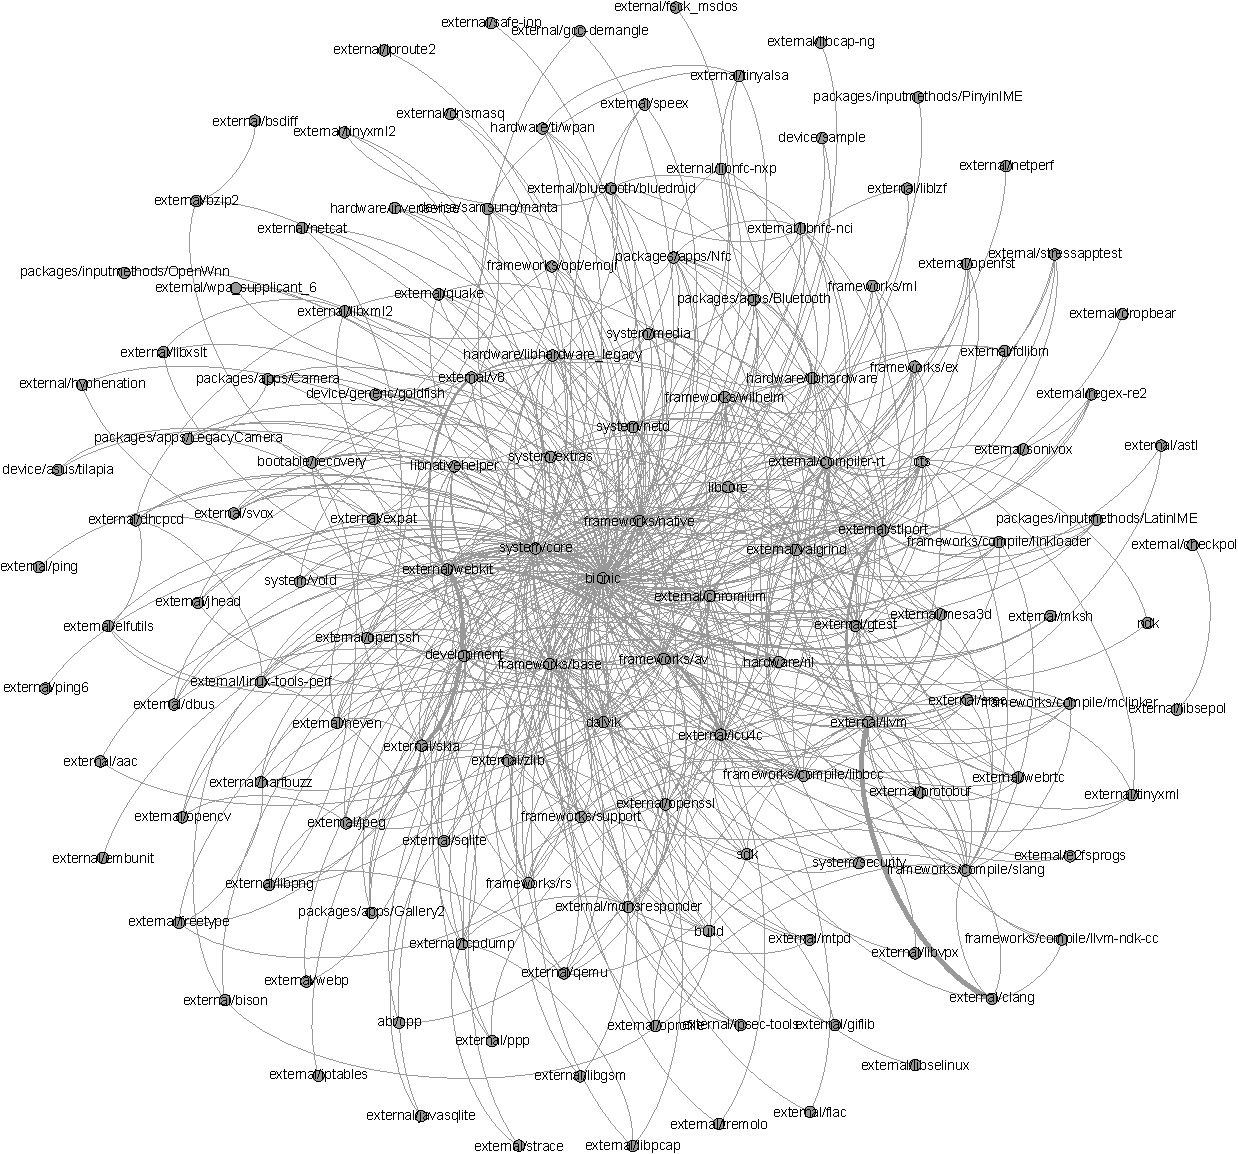
\includegraphics[width=0.9\linewidth]{callgraph.pdf}
   \caption{Граф межпакетных вызовов ОС Android 4.2}\label{pic:callgraph}
\end{figure}

\section{Методика тестирования}

Для тестирования использовался сервер, конфигурация которого описана в таблице \ref{table:test-server}:

\begin{table} [htbp]
  \centering
  \parbox{15cm}{\caption{Характеристики тестового стенда}\label{table:test-server}}
%  \begin{center}
  \begin{tabular}{| p{0.6\linewidth} || p{0.3\linewidth} |}
  \hline
  \hline
  Характеристика   & Значение \\
  \hline
  \hline
  Модель процессора   & Intel Xeon E5-2600 2.60 ГГц \\
  \hline
  Количество физических процессоров & 2   \\
  \hline
  Количество физических ядер процессора      & 8    \\
  \hline
  Количество виртуальных ядер процессора  & 16 (Hyper-Threading)   \\
  \hline
  Количество виртуальных ядер системы & 32   \\
  \hline
  Объём оперативной памяти & 96 Гб \\
  \hline
  Тип оперативной памяти & DDR3 \\
  \hline
  \hline
  \end{tabular}
%  \end{center}
\end{table}

Процессы анализаторов запускались параллельно на всех виртуальных процессорах. Время анализа измерялось от момента старта фазы анализа до момента завершения последнего процесса анализатора и выдачи финального отчёта.

В качестве базовой версии Clang Static Analyzer использовалась версия 3.4.1.

Анализатор (Clang Static Analyzer) имеет ряд настроек, непосредственно влияющих как на качество анализа, так и на его время. Ниже в таблице \ref{table:test-settings} перечислены опции анализатора, при которых производилось сравнение.

\begin{table} [htbp]
  \centering
  \parbox{15cm}{\caption{Тестовые настройки анализатора}\label{table:test-settings}}
%  \begin{center}
  \begin{tabular}{| p{0.35\linewidth} || p{0.35\linewidth} | p{0.2\linewidth} |}
  \hline
  \hline
  Имя параметра  & Назначение параметра & Значение \\
  \hline
  \hline
  \texttt{mode}   & Режим анализа. Влияет на максимальный размер функции, для которой выполняется анализ вложенного вызова & \texttt{deep} \\
  \hline
  \texttt{c++-inlining} & Анализ вызовов членов классов (C++) & \texttt{destructors}   \\
  \hline
  \texttt{cfg-temporary-dtors}   & Анализ вызовов деструкторов временныз объектов  & \texttt{false}    \\
  \hline
  \texttt{c++-stdlib-inlining} & Анализ вызовов стандартной библиотеки C++ & \texttt{true}   \\
  \hline
  \texttt{ipa-always-inline-size} & Размер функций, для которых всегда выполняется МПА & 3   \\
  \hline
  \texttt{c++-allocator-inlining} & Анализ аллокаторов (C++) & \texttt{false}   \\
  \hline
  \texttt{c++-template-inlining} & Анализ шаблонов функций (C++) & \texttt{true}   \\
  \hline
  \texttt{c++-container-inlining} & Анализ контейнерных классов (C++) & \texttt{true}   \\
  \hline
  \texttt{c++-shared\_ptr-inlining} & Анализ указателей \texttt{shared\_ptr} (C++) & \texttt{false}   \\
  \hline
  \texttt{max-times-inline-large} & Максимальное количество анализа вложенного вызова функции & 32   \\
  \hline
  \texttt{max-nodes} & Максимальное количество анализируемых узлов графа выполнения функции & \textit{варьируется}   \\
  \hline
  \hline
  \end{tabular}
%  \end{center}
\end{table}

Параметр \texttt{max-nodes} непосредственно влияет на полноту анализа, поэтому в дальнейшем измерения будут проходить с его учётом. Он станет одним из варьируемых параметров.

\section{Тестирование покрытия и производительности}

В качестве критерия производительности при сравнении межпроцедурного анализа методом встраивания и методом резюме можно взять количество узлов графа выполнения, обрабатываемых в единицу времени. Данный параметр может использоваться для режима встраивания непосредственно, однако для режима резюме он не отражает реальной производительности системы, поскольку каждому из узлов применения резюме в результирующем графе выполнения соответствует полноценный путь внутри одной или нескольких функций. Однако, количество узлов графа, соответствующих узлам применения резюме, можно вычислить рекурсивно, способом, схожим со способом построения отчёта при вложенном вызове функции: 

\begin{enumerate}
 \item Установить начальный счётчик узлов \texttt{cnt} = 0
 \item Пусть $N$~--- узел применения резюме, $M$~--- узел графа выполнения функции, на который хранится указатель в $N$
 \item Пока $M$~--- не корневой узел графа выполнения:
  \begin{enumerate}
   \item Увеличить \texttt{cnt} на 1
   \item Если $M$~--- узел применения резюме, выполнить для $M$ шаги алгоритма 1--3
   \item Установить $M$ равным родительскому узлу
  \end{enumerate}
\end{enumerate}

Таким образом, можно осуществить подсчёт количества \textit{эквивалентных} узлов графа выполнения, обрабатываемых в единицу времени. Поскольку для подсчёта используется только первый узел применения резюме, данный метод подсчёта даёт нижнюю границу количества обработанных узлов. Результаты измерения нижней границы для ОС Android представлены в таблице \ref{table:time-number}.

\begin{table}
%\setlength{\tabcolsep}{4pt}
\renewcommand{\arraystretch}{1.2}
\begin{tabular}{| l | p{0.13\linewidth} | p{0.15\linewidth} | p{0.2\linewidth} || p{0.2\linewidth} |}
\hline
Лимит количества узлов & Время анализа & Количество проанализированных узлов графа & Узлов графа в~секунду \\
\hline
\hline
8000      &   0:11       & $2,05 \cdot 10^8$  & $3,11 \cdot 10^5$ \\
\hline
16000     &   0:17       & $3,89 \cdot 10^8$  & $3,81 \cdot 10^5$ \\
\hline
32000     &   0:28       & $7,29 \cdot 10^8$  & $4,34 \cdot 10^5$ \\
\hline
64000     &   0:50       & $1,36 \cdot 10^9$  & $4,54 \cdot 10^5$ \\
\hline
128000    &   1:30       & $2,55 \cdot 10^9$  & $4,73 \cdot 10^5$ \\
\hline
256000    &   2:51       & $4,79 \cdot 10^8$  & $4,66 \cdot 10^5$ \\
\hline
512000    &   5:27       & $9,02 \cdot 10^8$  & $4,60 \cdot 10^5$ \\
\hline
\hline

\end{tabular}
\caption{Результаты измерений количества узлов графа, обрабатываемых в единицу времени, при внутримодульном анализе для метода встраивания} \label{table:time-number}
\end{table}


\begin{table}
%\setlength{\tabcolsep}{4pt}
\renewcommand{\arraystretch}{1.2}
\begin{tabular}{| l | p{0.13\linewidth} | p{0.15\linewidth} | p{0.2\linewidth} || p{0.2\linewidth} |}
\hline
Лимит количества узлов & Время анализа & Количество проанализированных узлов графа & Узлов графа в~секунду \\
\hline
\hline
2000      &   0:09       & $1,92 \cdot 10^8$  & $3,56 \cdot 10^5$ \\
\hline
4000      &   0:12       & $3,59 \cdot 10^8$  & $4,98 \cdot 10^5$ \\
\hline
8000      &   0:19       & $6,75 \cdot 10^8$  & $5,92 \cdot 10^5$ \\
\hline
16000     &   0:32       & $1,23 \cdot 10^9$  & $6,43 \cdot 10^5$ \\
\hline
32000     &   0:52       & $2,32 \cdot 10^9$  & $7,42 \cdot 10^5$ \\
\hline
64000     &   1:38       & $4,50 \cdot 10^8$  & $7,65 \cdot 10^5$ \\
\hline
128000    &   3:00       & $8,67 \cdot 10^8$  & $8,03 \cdot 10^5$ \\
\hline
\hline

\end{tabular}
\caption{Результаты измерений количества узлов графа, обрабатываемых в единицу времени, при внутримодульном анализе для метода резюме} \label{table:time-number}
\end{table}



\begin{table}
\renewcommand{\arraystretch}{1.2}
\begin{tabular}{| p{0.2\linewidth} | p{0.13\linewidth} | p{0.35\linewidth} | p{0.18\linewidth} |} 
\hline
Лимит количества узлов & Время анализа & Количество проанализированных узлов графа & Узлов графа в~секунду \\
\hline
\hline
8000      &   0:26       & $1,58 \cdot 10^8$  & $1,01 \cdot 10^5$ \\
\hline
16000     &  0:33        & $3,09 \cdot 10^8$  & $1,56 \cdot 10^5$ \\
\hline
32000     &  0:47        & $5,96 \cdot 10^8$  & $2,11 \cdot 10^5$ \\
\hline
64000     &  1:13        & $1,14 \cdot 10^9$  & $2,60 \cdot 10^5$ \\
\hline
128000    &   2:07       & $2,18 \cdot 10^9$  & $2,86 \cdot 10^5$ \\
\hline
256000    &   3:56       & $4,22 \cdot 10^8$  & $2,98 \cdot 10^5$ \\
\hline
\hline

\end{tabular}
\caption{Результаты измерений количества узлов графа, обрабатываемых в единицу времени, при межмодульном анализе для метода встраивания} \label{table:time-nodes-xtu-inlining}

\end{table}


\begin{table}
\renewcommand{\arraystretch}{1.2}
\begin{tabular}{| p{0.2\linewidth} | p{0.13\linewidth} | p{0.35\linewidth} | p{0.18\linewidth} |} 
\hline
Лимит количества узлов & Время анализа & Количество проанализированных узлов графа & Узлов графа в~секунду \\
\hline
\hline
2000      &   0:28       & $4,01 \cdot 10^8$  & $2,38 \cdot 10^5$ \\
\hline
4000      &   0:41       & $7,54 \cdot 10^8$  & $3,06 \cdot 10^5$ \\
\hline
8000      &   0:53       & $1,40 \cdot 10^9$  & $4,40 \cdot 10^5$ \\
\hline
16000     &  1:23        & $2,85 \cdot 10^9$  & $5,72 \cdot 10^5$ \\
\hline
32000     &  2:18        & $5,43 \cdot 10^9$  & $6,55 \cdot 10^5$ \\
\hline
64000     &  4:41        & $1,07 \cdot 10^{10}$ & $6,34 \cdot 10^5$ \\
\hline
\hline

\end{tabular}
\caption{Результаты измерений количества узлов графа, обрабатываемых в единицу времени, при межмодульном анализе для метода резюме} \label{table:time-nodes-xtu-summary}

\end{table}
